\documentclass[aspectratio=169, 11pt]{beamer}

% -------------------------------------------------------
% Theme (matching prior deck: Madrid/whale, dark header)
% -------------------------------------------------------
\usetheme{Madrid}
\usecolortheme{whale}

\definecolor{darkheader}{RGB}{44,62,80}
\definecolor{accentcol}{RGB}{52,152,219}
\definecolor{greencol}{RGB}{39,174,96}
\definecolor{redcol}{RGB}{192,57,43}

\setbeamercolor{frametitle}{bg=darkheader, fg=white}
\setbeamercolor{title}{bg=darkheader, fg=white}
\setbeamercolor{structure}{fg=darkheader}
\setbeamercolor{block title}{bg=darkheader, fg=white}
\setbeamercolor{block body}{bg=darkheader!8, fg=black}
\setbeamercolor{block title alerted}{bg=accentcol!80, fg=white}
\setbeamercolor{block body alerted}{bg=accentcol!10, fg=black}
\setbeamercolor{block title example}{bg=greencol!80, fg=white}
\setbeamercolor{block body example}{bg=greencol!10, fg=black}
\setbeamercolor{alerted text}{fg=accentcol}

\setbeamertemplate{navigation symbols}{}
\setbeamertemplate{footline}[frame number]

% -------------------------------------------------------
% Packages
% -------------------------------------------------------
\usepackage{amsmath, amssymb, amsthm, mathtools}
\usepackage{bm}
\usepackage{booktabs}
\usepackage{tikz}
\usetikzlibrary{arrows.meta, positioning, calc, decorations.pathreplacing}
\usepackage{natbib}

% -------------------------------------------------------
% Math macros
% -------------------------------------------------------
\newcommand{\E}{\mathbb{E}}
\newcommand{\R}{\mathbb{R}}
\newcommand{\Fcal}{\mathcal{F}}
\newcommand{\med}{\mathrm{med}}
\newcommand{\zt}{\mathbf{z}(t)}
\newcommand{\bt}{\bm{\beta}}
\newcommand{\lam}{\lambda}
\newcommand{\Ncal}{\mathcal{N}}
\newcommand{\eps}{\varepsilon}

% -------------------------------------------------------
% Title
% -------------------------------------------------------
\title[News Encoders \& Macro Expectations]{Reconstructing Macroeconomic Expectations\\via Financial News Encoders}
\subtitle{A FinBERT-Based Pipeline for Survey Expectation Extrapolation}
\author{Aaron Huberman \and Rafael Alves}
\institute{Duke University}
\date{\today}

% -------------------------------------------------------
% Document
% -------------------------------------------------------
\begin{document}

% ============================================================
% TITLE SLIDE
% ============================================================
\begin{frame}
  \titlepage
\end{frame}

% ============================================================
% OUTLINE
% ============================================================
\begin{frame}{Outline}
  \tableofcontents
\end{frame}

% ============================================================
\section{Motivation}
% ============================================================

\begin{frame}{Why Do We Need Historical Expectations?}

Survey-based expectation data (SPF, Michigan Survey, Blue Chip) is:
\begin{itemize}\itemsep2pt
  \item \textbf{Temporally thin} --- the SPF begins in 1968Q4, Blue Chip in the 1970s
  \item \textbf{Low frequency} --- quarterly or monthly, limiting time-series power
  \item \textbf{Cross-sectionally sparse} --- micro-data panels are small relative to rich text corpora
\end{itemize}

\vspace{0.3cm}
\textbf{Why this matters for macro-finance.}
\begin{itemize}\itemsep2pt
  \item Structural SDF estimation under heterogeneous beliefs requires \emph{long} expectation series
  \item Carroll (2003) requires a professional forecast anchor --- we need this pre-1968
  \item Pricing kernel non-monotonicity tests are underpowered on short panels
\end{itemize}

\vspace{0.3cm}
\begin{block}{This Paper}
We use financial news embeddings to project survey-consistent expectations \emph{backward in time}, calibrated on the overlap period between surveys and the news archive.
\end{block}

\end{frame}

% ============================================================
\section{Core Idea}
% ============================================================

\begin{frame}{The Central Insight}

\begin{alertblock}{Key Assumption}
If the information environment determines beliefs, encoding the news that survey respondents read should recover the median respondent's forecast --- and allow us to extend it through history.
\end{alertblock}

\vspace{0.3cm}
\textbf{Two competing approaches:}

\vspace{0.2cm}
\begin{columns}
\begin{column}{0.48\textwidth}
  \begin{block}{\textcolor{redcol}{$\times$} Fine-tune LLM}
    \begin{itemize}\itemsep2pt
      \item Train LLM to match median survey forecast
      \item Underdetermined: too few survey waves
      \item Black-box; breaks on distribution shift
    \end{itemize}
  \end{block}
\end{column}
\begin{column}{0.48\textwidth}
  \begin{exampleblock}{\textcolor{greencol}{$\checkmark$} Frozen Encoder + Ridge}
    \begin{itemize}\itemsep2pt
      \item Freeze pretrained FinBERT encoder
      \item Aggregate embeddings per survey wave
      \item Ridge: $\zt \mapsto$ median forecast
      \item Apply fitted map to pre-survey news
    \end{itemize}
  \end{exampleblock}
\end{column}
\end{columns}

\end{frame}

% ============================================================
\section{Pipeline}
% ============================================================

\begin{frame}{Pipeline Overview}

\begin{center}
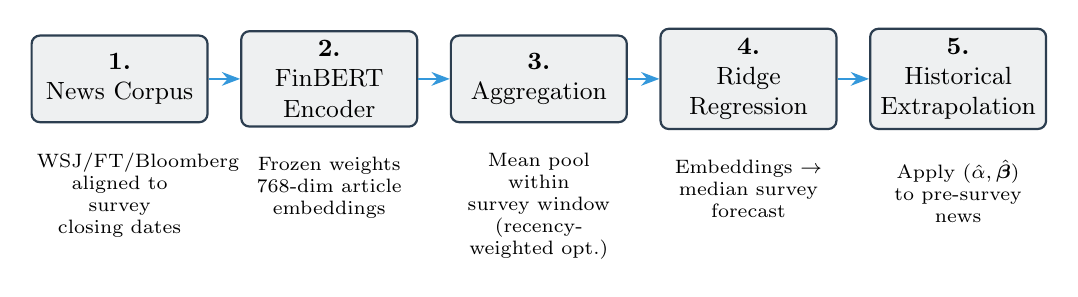
\begin{tikzpicture}[
  node distance=0.55cm and 0.4cm,
  box/.style={rectangle, draw=darkheader, thick, rounded corners=3pt,
              fill=darkheader!8, text width=2.0cm, align=center,
              minimum height=1.1cm, font=\small},
  arr/.style={-Stealth, thick, color=accentcol}
]

\node[box] (news)  {\textbf{1.}\\ News Corpus};
\node[box, right=of news] (enc)   {\textbf{2.}\\ FinBERT\\ Encoder};
\node[box, right=of enc]  (agg)   {\textbf{3.}\\ Aggregation};
\node[box, right=of agg]  (reg)   {\textbf{4.}\\ Ridge\\ Regression};
\node[box, right=of reg]  (ext)   {\textbf{5.}\\ Historical\\ Extrapolation};

\draw[arr] (news) -- (enc);
\draw[arr] (enc)  -- (agg);
\draw[arr] (agg)  -- (reg);
\draw[arr] (reg)  -- (ext);

\node[below=0.25cm of news, font=\scriptsize, text width=2.1cm, align=center]
  {WSJ/FT/Bloomberg\\ aligned to survey\\ closing dates};
\node[below=0.25cm of enc, font=\scriptsize, text width=2.1cm, align=center]
  {Frozen weights\\ 768-dim article\\ embeddings};
\node[below=0.25cm of agg, font=\scriptsize, text width=2.1cm, align=center]
  {Mean pool within\\ survey window\\ (recency-weighted opt.)};
\node[below=0.25cm of reg, font=\scriptsize, text width=2.1cm, align=center]
  {Embeddings $\to$\\ median survey\\ forecast};
\node[below=0.25cm of ext, font=\scriptsize, text width=2.1cm, align=center]
  {Apply $(\hat{\alpha},\hat{\bt})$\\ to pre-survey\\ news};

\end{tikzpicture}
\end{center}

\vspace{0.2cm}
\begin{block}{Validation Protocol}
Reserve the most recent $K$ survey waves as a hold-out. Evaluate RMSE and directional accuracy \emph{before} applying the map to the pre-survey historical record.
\end{block}

\end{frame}

% ============================================================
\begin{frame}{Why Not Fine-Tune the LLM?}

The original proposal (Rafael) was to fine-tune an LLM so that its average forecast over news articles matches the median survey respondent.

\vspace{0.3cm}
\textbf{Three problems with this approach:}

\begin{enumerate}
  \item \textbf{Identification.} The survey yields one scalar per wave --- far too few observations to constrain 7B+ parameters. Even with aggressive regularization, there is no guarantee the learned behavior generalizes.

  \item \textbf{Overfitting in the extrapolation.} If the model has memorized the calibration mapping, applying it to 1960s WSJ articles --- which are stylistically, lexically, and informationally very different --- produces answers with no validity guarantee.

  \item \textbf{Interpretability.} A frozen encoder + ridge regression has a clean identification story: the feature space is fixed exogenously, and the regression coefficients are the only free parameters. Reviewers understand this. A fine-tuned LLM does not have a clear identification narrative.
\end{enumerate}

\vspace{0.1cm}
\begin{alertblock}{Key observation}
Once you have the textual encoder, the problem reduces to a standard high-dimensional regression. The LLM wrapper adds complexity without payoff.
\end{alertblock}

\end{frame}

% ============================================================
\section{Encoder \& Regression}
% ============================================================

\begin{frame}{Encoder Choice: FinBERT}

\textbf{Recommended for proof of concept:} \texttt{ProsusAI/finbert} (HuggingFace)

\vspace{0.3cm}
\begin{columns}
\begin{column}{0.55\textwidth}
  \begin{tabular}{ll}
    \toprule
    Property & Detail \\
    \midrule
    Architecture & BERT-base, 768-dim \\
    Pretraining & Financial news + SEC filings \\
    Fine-tuning & None --- frozen throughout \\
    Compute & CPU-friendly; fast on RTX 5070 Ti \\
    Literature & Standard in empirical finance \\
    \bottomrule
  \end{tabular}
\end{column}
\begin{column}{0.42\textwidth}
  \begin{block}{Why Frozen?}
    \begin{itemize}
      \item No leakage of survey targets into feature space
      \item Dimensionality fixed at 768 --- tractable given limited survey wave count
      \item Stability across time periods critical for extrapolation validity
    \end{itemize}
  \end{block}
\end{column}
\end{columns}

\vspace{0.4cm}
\textbf{Longer-term upgrade path:}
\begin{itemize}
  \item RoBERTa-based financial encoders (e.g.\ \texttt{yiyanghkust/finbert-tone})
  \item Domain-adapted encoder trained on FOMC statements + macro news
  \item Validate improvement on calibration hold-out before switching
\end{itemize}

\end{frame}

% ============================================================
\begin{frame}{Regression Specification}

\textbf{For each survey wave $t$}, construct the aggregate embedding:
\[
  \zt = \frac{1}{|A_t|} \sum_{a \in A_t} \phi_{\text{FinBERT}}(a) \;\in\; \R^{768}
\]
where $A_t$ is the set of articles published before the wave $t$ closing date.

\vspace{0.4cm}
\textbf{Calibration regression:}
\[
  \boxed{\med_t = \alpha + \bt^\top \zt + \eps_t}
\]
with $\med_t$ the median survey forecast (e.g.\ SPF 1-year CPI), and $\bt \in \R^{768}$ estimated via Ridge:
\[
  (\hat{\alpha}, \hat{\bt}) = \arg\min_{\alpha, \bt} \sum_{t \in \mathcal{T}_{\text{cal}}} \left(\med_t - \alpha - \bt^\top \zt\right)^2 + \lam \|\bt\|^2
\]

\textbf{Penalty selection:} leave-one-out cross-validation over survey waves (not observations).

\vspace{0.3cm}
\begin{alertblock}{Identification}
The frozen encoder ensures $\zt$ is constructed entirely from text --- no information from $\med_t$ enters the feature space. The only free parameters are $(\alpha, \bt)$.
\end{alertblock}

\end{frame}

% ============================================================
\begin{frame}{Historical Extrapolation}

Once $(\hat{\alpha}, \hat{\bt})$ are validated in hold-out, apply to the pre-survey news record:

\[
  \widehat{\med}_t = \hat{\alpha} + \hat{\bt}^\top \zt, \qquad t \in \mathcal{T}_{\text{hist}}
\]

\vspace{0.3cm}
\textbf{Diagnostic checks before treating $\widehat{\med}_t$ as valid:}

\begin{enumerate}
  \item \textbf{Economic plausibility.} Do $\widehat{\med}_t$ spike around the Volcker disinflation (1979--83), GFC, and COVID? Do they track realized inflation at business cycle frequency?
  
  \item \textbf{Benchmark comparison.} Cross-validate against Livingston Survey (available from 1946) and Blue Chip (1970s+) where series overlap.

  \item \textbf{Embedding support check.} Are historical $\zt$ in-distribution relative to calibration-era embeddings? Compute the Mahalanobis distance of each historical embedding from the calibration cloud; flag out-of-support periods.

  \item \textbf{Sensitivity.} Vary aggregation window, recency weighting, and $\lam$ --- report a robustness table.
\end{enumerate}

\end{frame}

% ============================================================
\section{Preliminary Results}
% ============================================================

\begin{frame}{Preliminary Results}

\begin{center}
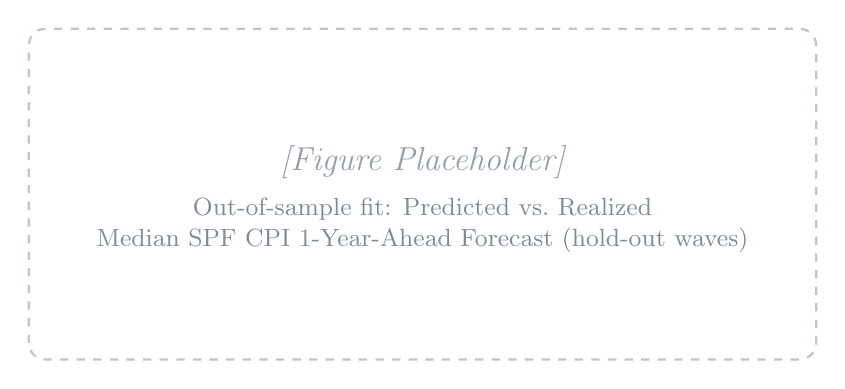
\begin{tikzpicture}
  \draw[darkheader!30, dashed, thick, rounded corners=6pt]
    (0,0) rectangle (10,4.2);
  \node[darkheader!50, font=\large\itshape] at (5, 2.5)
    {[Figure Placeholder]};
  \node[darkheader!60, font=\small, align=center] at (5, 1.7)
    {Out-of-sample fit: Predicted vs.\ Realized\\
     Median SPF CPI 1-Year-Ahead Forecast (hold-out waves)};
\end{tikzpicture}
\end{center}

\vspace{0.1cm}
\textbf{Planned results table:}
\begin{center}
\begin{tabular}{lccc}
  \toprule
  Model & RMSE & Dir.\ Accuracy & Benchmark \\
  \midrule
  AR(1) baseline & --- & --- & --- \\
  FinBERT Ridge & --- & --- & --- \\
  FinBERT + recency weights & --- & --- & --- \\
  \bottomrule
\end{tabular}
\end{center}

\end{frame}

% ============================================================
\section{Connection to Research Agenda}
% ============================================================

\begin{frame}{Connection to the Broader Research Agenda}

This pipeline is a \emph{measurement tool} that feeds into three broader projects:

\vspace{0.2cm}
\begin{enumerate}\itemsep4pt
  \item \textbf{Carroll (2003) Epidemiological Model.} \\
        Long-run professional forecast series anchors the diffusion process for household expectation updating. The current SPF is too short to estimate the diffusion parameter reliably.

  \item \textbf{FT Reader Comment Corpus Paper.} \\
        The synthetic series provides a structural macro baseline for benchmarking text-derived sentiment and disagreement measures.

  \item \textbf{Pricing Kernel and SDF Estimation.} \\
        Heterogeneous-beliefs SDF models require long series on belief dispersion. The pipeline can produce quantile-specific forecasts, proxying the cross-sectional distribution.
\end{enumerate}

\vspace{0.15cm}
\begin{alertblock}{Research Philosophy}
NLP/ML as \emph{measurement tool}, not primary contribution.
\end{alertblock}

\end{frame}

% ============================================================
\section{Conclusion}
% ============================================================

\begin{frame}{Summary and Next Steps}

\textbf{Summary:}
\begin{itemize}\itemsep1pt
  \item Survey expectation data is temporally thin; news corpora are dense and long
  \item A frozen FinBERT encoder + ridge regression provides a principled, interpretable mapping from the information environment to median survey forecasts
  \item Validated out-of-sample, the map reconstructs survey-consistent expectations through the archival news record
\end{itemize}

\vspace{0.2cm}
\textbf{Next steps:}
\begin{enumerate}\itemsep1pt
  \item Assemble WSJ article corpus aligned to SPF survey closing dates
  \item Run FinBERT encoding pipeline (RTX 5070 Ti)
  \item Fit ridge regression; tune $\lam$ by LOO-CV over waves
  \item Evaluate hold-out RMSE vs.\ AR(1) baseline
  \item If validated: extrapolate pre-1968; compare to Livingston Survey
\end{enumerate}

\vspace{0.15cm}
\begin{block}{Open Questions}
(i) Recency weighting for article aggregation. \;
(ii) Article-level vs.\ headline-level embeddings. \;
(iii) Structural breaks in the news--forecast mapping post-internet.
\end{block}

\end{frame}

% ============================================================
% REFERENCES
% ============================================================
\begin{frame}[allowframebreaks]{References}
\begin{itemize}\small
  \item Carroll, C.\ (2003). ``Macroeconomic expectations of households and professional forecasters.'' \textit{QJE}.
  \item Croushore, D.\ (1993). ``Introducing: The Survey of Professional Forecasters.'' \textit{Federal Reserve Bank of Philadelphia Business Review}.
  \item Harrison, J.\ \& Kreps, D.\ (1978). ``Speculative investor behavior in a stock market with heterogeneous expectations.'' \textit{QJE}.
  \item Livingston, J.\ (1946--). Livingston Survey. \textit{Federal Reserve Bank of Philadelphia}.
  \item Malo, P., Sinha, A., Korhonen, P., Wallenius, J., \& Takala, P.\ (2014). ``Good debt or bad debt: Detecting semantic orientations in economic texts.'' \textit{JASIST}. [FinBERT pretraining corpus]
  \item Tibshirani, R.\ (1996). ``Regression shrinkage and selection via the lasso.'' \textit{JRSS-B}.
\end{itemize}
\end{frame}

\end{document}
